\section{Аннотация}

\underline{Цель работы}: 
\begin{enumerate}
    \item Экспериментально получить распределение термоэлектронов по энергиям и скоростям
    \item Изучить зависимость распределений от температуры
\end{enumerate} \par
\underline{Оборудование}:
\begin{enumerate}
    \item Лампа 6Ф1П
    \item Тороидальный трансформатор и блок питания питания тока.
    \item Макетная плата, резисторы, диоды, конденсатор, провода, операционный усилитель.
    \item Arduino UNO
\end{enumerate} 
\newpage

\section{Теоретические сведения}
\subsection{Устройство радиолампы}

\underline{Описание:}
\par
Электронная лампа, радиолампа — электровакуумный прибор (точнее, вакуумный электронный прибор), работающий за счёт управления интенсивностью потока электронов, движущихся в вакууме или разрежённом газе между электродами.

\underline{Принцип работы:}
\par

Самая простая радиолампа имеет колбу, внутри которой размещены два электрода — катод и анод. Катод разогревается от источника тока до температуры, при которой из него вследствие термоэлектронной эмиссии могут вылетать электроны, и свободно перемещаться внутри вакуума колбы. Электроны имеют отрицательный заряд, и если на второй электрод, анод, будет подан положительный потенциал, электроны устремятся к аноду, попадут в него и создадут ток в цепи анод-катод. Если на анод подать отрицательный потенциал, то электроны, имея одноимённый заряд, будут отталкиваться от анода, и ток в цепи протекать не будет. Такая простая радиолампа называется кенотрон и пригодна для выпрямления переменного тока в постоянный ток, так как проводит ток только в одном направлении.

\par
Более сложная радиолампа — триод устроена так же, но имеет ещё и третий электрод — сетку, расположенную между анодом и катодом. Если потенциал на сетке отсутствует, а на аноде потенциал положительный, при этом примем потенциал катода за нуль, то все электроны, вылетевшие с катода, устремляются к аноду и создают ток в цепи анода. Если подать на сетку небольшой отрицательный потенциал, то она своим полем сможет отклонять часть электронов на пути к аноду, тем самым уменьшая ток анода. Чем больше по модулю отрицательный потенциал на сетке — тем большая часть электронов будет отклонена, тем меньше ток анода. Если подать на сетку достаточно большой отрицательный потенциал — то лампа окажется «заперта» — ток в цепи анода прекратится. Такая лампа может работать как усилитель, если подать на сетку слабый электрический сигнал, то он вызовет синхронные изменения тока анода, причем на ощутимо большие величины.


\underline{Применение:}
\par
Радиолампы массово использовались в XX веке как основные элементы радиоаппаратуры, так как позволяют выпрямлять ток, усиливать, генерировать электрические сигналы и т. п.

Электронные лампы до сих пор находят применение в аудиотехнике, как любительской, так и профессиональной. Конструирование ламповых звукотехнических устройств является одним из направлений современного радиолюбительского движения.

Благодаря специфическим особенностям искажения, которые до настоящего времени не удалось полностью воспроизвести в широкой практике при использовании полупроводниковых аналогов или цифровой эмуляции, электронные лампы весьма популярны в усилении звучания электрогитары.

\subsection{Распределение}

Для описания поведения систем, состоящих из большого числа частиц, обычно применяется 
статистический подход, одним из основных понятий которого является понятие плотности 
распределения вероятности. Пусть, например, в некотором объеме содержится $N$ молекул 
газа, находящихся в состоянии непрерывного хаотического движения. Положение в 
пространстве и скорость каждой из молекул с течением времени изменяются случайным 
образом, такие величины принято называть случайными. Предположим, что нам удалось 
измерить скорости $V_i$ всех молекул в некоторый момент времени. Тогда для любого 
бесконечно малого интервала скоростей $dv$ можно найти число $dN$ молекул, для которых 
значение скорости находится в интервале от $v$ до $v + dv$, причем $dN$ будет пропорционально 
величине интервала $dv$ и общему числу молекул $N$:  
\begin{equation}
    dN = N \cdot f(v) \cdot dv
\end{equation}
Коэффициент пропорциональности $f(v)$ называют плотностью распределения
вероятности скорости V молекул.
\par
При N $\rightarrow \infty $ отношение $\frac{dN}{N}$ стремится к вероятности $P$ того, что для
любой частицы значение случайной величины $v$ попадет в соответствующий
интервал, т.е. 
\begin{equation}
    P(v \leq V \leq v + dv) = f(v) \cdot dv
\end{equation}
Или
\begin{equation}
    dP(v) = f(v) \cdot dv
\end{equation}
Так как вероятность любого события лежит в интервале от нуля до
единицы, плотность распределения удовлетворяет условиям:
\[f(v) \geq 0 \text{ и } \int_{0}^{\infty} f(v)dv = 1 - \text{условие нормировки}\]

\par 
Для нахождения вероятности того, что значение случайной величины $v$
попадет в произвольный интервал $(v1,v2)$ , необходимо вычислить интеграл
\begin{equation}
    P(v_1 \leq V \leq v_2) = \int_{v_1}^{v_2} f(v)dv
\end{equation}

\par 
Наивероятнейшим значением случайной величины называют значение,
соответствующее максимуму плотности распределения вероятности:
\[f(v_\text{наив} ) = max f(v); (0 <  v  < \infty)\]

\par 
Среднее значение $\langle$V$\rangle$ случайной величины $v$ можно найти по формуле:
\begin{equation}
    \langle V \rangle = \int_{0}^{\infty} v \cdot f(v) \cdot dv
\end{equation}

\par
Аналогичным образом находится и среднее значение какой-либо функции
от случайной величины. Например, среднее значение кинетической энергии 
$\text{E}_\text{кин} =  \frac{mv^2}{2}$ молекул равно:
\begin{equation}
    \langle E_{\text{кин}} \rangle = \int_{0}^{\infty} \frac{mv^2}{2} \cdot f(v) \cdot dv
\end{equation}

\par 
Случайной величиной является не только модуль скорости $v$, но и ее
проекции $V_x , V_y ,V_z $ на оси координат, в этом случае можно записать:
\[dP(v_x, v_y, v_z) = f(v_x, v_y, v_z) \cdot 
dv_x \cdot dv_y \cdot dv_z, \]
где  $v_x,v_y ,v_z$ - вероятность того, что $х$-компонента $v_{x}$ скорости электрона лежит в интервале от $v_x$ до $v_x + dv_{x} $, $y$-компонента $V_y$ скорости электрона лежит в интервале от $v_y$ до $v_y + dv_y$ , $z$-компонента $V_z$ скорости электрона лежит в интервале от $v_z $ до $v_z +  dv_z$ :
\[dP (v_x,v_y ,v_z ) = P (v_x \leq V_x \leq v_x + dv_x ,v_y \leq V_y \leq v_y + dv_y ,v_z \leq V_z \leq v_z + dv_z ).\]

\par 
Для реальных физических термодинамических систем информацию о плотности
распределения получают как результат обобщения большого числа
экспериментальных данных, на базе которых строятся математические модели
явления. В настоящей работе изучается распределение по скоростям и по
энергиям термоэлектронов, вылетающих из нагретой нити накала электронной
лампы.

\subsection{Статистическое описание поведения электронов в металле}
\par 
В
соответствии с электронной теорией металлов их отличительные свойства
объясняются наличием в них оторванных от атомов электронов, хаотически
перемещающихся по всему объему металла. Когда электрон подлетает к границе
между металлом и вакуумом, равнодействующая всех сил, действующих на
электрон, направлена вглубь металла и мешает ему покинуть металл. Однако,
если скорость движения и, следовательно, кинетическая энергия электрона
достаточно велика, то он способен вылететь из металла. Энергия, затрачиваемая
на отрыв электрона от металла, называется работой выхода. Чем выше 
температура металла, тем больше доля электронов, обладающих энергией,
превышающей работу выхода, и, следовательно, тем больше число вылетающих
электронов. Это явление носит название термоэлектронной эмиссии.

Распределение по скоростям
вылетевших из металла электронов имеет вид: 
\begin{equation}
    dP(v_x, v_y, v_z)  = (\frac{m}{2\pi kT})^{\frac{3}{2}} \cdot exp(-\frac{m(v_{x}^{2} + v_{y}^{2} + v_{z}^{2})}{2kT})\cdot dv_{x} dv_{y}dv_{z}
\end{equation}
где $m$ – масса электрона; $T$- температура электронного газа.
\par 
В данном случае плотность распределения f($v_x, v_y, v_z$) является
трехмерной функцией в декартовых координатах $v_x, v_y, v_z$:
\[f(v_x, v_y, v_z) = (\frac{m}{2\pi kT})^{\frac{3}{2}} \cdot exp(-\frac{m(v_{x}^{2} + v_{y}^{2} + v_{z}^{2})}{2kT})\]
Эта формула совпадает с формулой для распределения Максвелла, которое
описывает распределение молекул по скоростям в идеальном газе при
температуре $Т$. Таким образом, можно утверждать, что вылетевшие электроны у
поверхности металла подчиняются распределению Максвелла.
Чтобы найти распределение электронов по модулю скорости $dP(v)$,
необходимо перейти в (7) к сферическим координатам v, $\phi, \theta$, заменив элемент
"объема" $dv_xdv_ydv_z$ в декартовых координатах на соответствующий элемент
$v^2sin\theta dv d \phi d \theta $ в сферических координатах:

\[dP(v, \phi, \theta) = (\frac{m}{2\pi kT})^{\frac{3}{2}} \cdot exp(-\frac{mv^2}{2kT}) v^2 sin \theta dv d \phi d \theta \]

Интеграл по "не интересующим" переменным $\phi$ и $\theta$ дает:

\[\int_{0}^{2\pi}d\phi \int_{0}^{\pi}sin\theta \cdot d\theta = 4\pi\]

в результате получим
\begin{equation}
    dP(v) = 4\pi (\frac{m}{2\pi kT})^{\frac{3}{2}} \cdot exp(-\frac{mv^2}{2kT}) v^2 dv
\end{equation}

\par 
Распределение электронов по энергии можно получить, сделав замену
переменных
\[E_{\text{кин}} = \frac{mv^2}{2}\]

при этом

\[dE = mvdv v^2dv = \sqrt{\frac{2E_{\text{кин}}}{m^3}}dE_{кин}\]
В итоге получаем:
\[dP(E_{\text{кин}}) = \frac{2}{\sqrt{\pi}kT}\cdot \sqrt{\frac{E_{\text{кин}}}{kT}} \cdot exp(-\frac{E_{\text{кин}}}{kT})dE_{\text{кин}}\]

Таким образом, плотность распределения по энергии f($Е_{\text{кин}}$) равна
\begin{equation}
    df(E_{\text{кин}}) = \frac{2}{\sqrt{\pi}kT}\cdot \sqrt{\frac{E_{\text{кин}}}{kT}} \cdot exp(-\frac{E_{\text{кин}}}{kT})
\end{equation}

\par 
Можно найти среднее значение кинетической энергии электрона $\langle E_{\text{кин}} \rangle$ ,
вылетевшего из катода:

\[\langle E_{\text{кин}} \rangle = \int_{0}^{\infty}E_{\text{кин}}\cdot f(E_{\text{кин}}) \cdot dE_{\text{кин}} = \frac{3}{2}kT\]
(такой же результат можно получить и при вычислениях по формуле (6)).
\par 
Для температуры катода порядка 1000 К средняя энергия термоэлектронов
составляет доли электронвольта. В свою очередь, энергия электронов внутри
металла примерно составляет 5-10 эВ. Однако термодинамическая температура
электронов внутри и вне металла одна и та же и равна температуре катода, так как
система находится в термодинамическом равновесии. Это связано с различной
статистикой распределения электронов внутри и вне металла.

\subsection{Экспериментальное изучение распределения термоэлектронов}

\par
Для изучения распределения термоэлектронов, вылетающих из металла,
необходимо провести эксперимент, схема которого позволяла бы каким-либо
способом сортировать термоэлектроны по скорости. Рассмотрим процессы,
происходящие в диоде - электронной лампе, представляющей собой
цилиндрический анод, на оси которого расположена тонкая нить - катод. При
нагревании катода начинается процесс термоэлектронной эмиссии. Электроны от
катода устремляются к аноду, и, если анод и катод замкнуть в цепь через
амперметр, то прибор зафиксирует появление тока.
\par Включим в цепь между анодом и катодом регулируемый источник
напряжения. Если на анод подать отрицательное напряжение $U<0$ относительно
катода, то до анода смогут долететь только те электроны, для которых величина
$E_r = \frac{mv_{r}^{2}}{2} = \frac{m(v_{x}^{2} + v_{y}^{2})}{2}$ больше $е|U|>0$. По мере увеличения напряжения число
электронов, долетающих до анода, и, следовательно, ток в цепи будут возрастать,
и если бы электроны не взаимодействовали друг с другом, то при $U=0$ они все
долетали бы до анода, ток достиг бы максимального значения и не изменялся бы
при дальнейшем увеличении напряжения.
\par
Найдем зависимость анодного тока от величины приложенного
напряжения $U<0$ при условии, что термоэлектроны вылетают из катода в
соответствии с распределением Максвелла и по пути к аноду не
взаимодействуют. Сначала получим формулу, описывающую распределение
электронов по радиальной компоненте скорости $v_r$. Для этого в (7) перейдем к
цилиндрическим координатам, заменив $dv_x dv_y dv_z$ на $v_r dv_r d\phi dv_z$ , тогда:
\[dP(v_r, \phi, v_z) = (\frac{m}{2\pi kT})^{\frac{3}{2}} \cdot exp(-\frac{m(v_{r}^{2} + v_{z}^{2}}{2kT}) v_r dv_r d \phi dv_z \]

\par 
Интегрируя по $d\phi dv_z$, получим:
\begin{equation}
    dP(v_r) = 2\pi v_r (\frac{m}{2\pi kT}) \cdot exp(-\frac{mv_{r}^{2}}{2kT}) dv_r = \frac{m}{kT} \cdot exp(-\frac{mv_{r}^{2}}{2kT}) \cdot v_r dv_r
\end{equation}
\par 
Плотность тока $dj(v_r)$ в поперечном сечении $S$, примыкающем к катоду,
создаваемая электронами, радиальная компонента скорости которых лежит в
интервале от $v_r$ до $v_r + dv_r$, задается формулой:

\begin{equation}
    dj(v_r) = \frac{dq(v_r)}{Sdt} = \frac{e \cdot v_r \cdot S  \cdot dt \cdot dn(v_r)}{S \cdot dt} = e \cdot v_r \cdot dn(v_r) = e \cdot v_r \cdot  n_0 \cdot dP(v_r)
\end{equation}
где  $dn(v_r)$ - концентрация электронов с соответствующими скоростями; $e$ - 
заряд
электрона; $S$ – площадь поперечного сечения; $n_0$ - концентрация электронов
вблизи катода.
Чтобы найти плотность тока j(U) в зависимости от анодного напряжения
$U<0$, необходимо проинтегрировать выражение (11) по $v_r$, удовлетворяющим
условию $\frac{mv_{r}^{2}}{2} > е|U|$:
\[j(U) = e n_0 \cdot \int_{\sqrt{\frac{2e|U|}{m}}}^{\infty} (\frac{m}{kT})\cdot 
exp(-\frac{mv_{r}^{2}}{2kT})\cdot v_{r}^{2} dv_{r}\]

\par
Интегрируя по частям, получим окончательно для плотности тока при
$U<0$:
\begin{equation}
    j_{a}(U)=j_0 \cdot \frac{2}{\sqrt{\pi}}
    \left[
    (\frac{e|U|}{kT})^{\frac{1}{2}}exp(-\frac{e|U|}{kT})+ \int_{(\frac{e|U|}{kT})^{\frac{1}{2}}}^{\infty}exp(-x^2)dx
    \right],
\end{equation}

где $j_0$ - плотность тока насыщения, устанавливающаяся в лампе при U>0:

\[j_0 = \frac{en_0}{2}\sqrt{\frac{2 \pi kT}{m}}\]

Зависимость анодного тока $I_a$, равного произведению плотности тока (12) на
площадь катода, изображена на рис.\ref{fig:zavis_toka}.

Продифференцировав выражение (12) по U, получим зависимость
производной $dI_a/dU$ от $U<0$ в виде рис.\ref{fig:zavis_proizv} :

\begin{equation}
    \frac{dI_a}{dU} = C^{''}\cdot
    \left[
    \sqrt{\frac{e|U|}{kT}} \cdot exp(-\frac{e|U|}{kT})
    \right]
\end{equation}

Тогда наша зависимость имеет вид:

\begin{equation}
    \frac{dI_a}{dU} = -ab \cdot
    \left[
    \sqrt{b|U|} \cdot exp(-b|U|)
    \right]
    \label{major_func}
\end{equation}

где $a = j_0 \cdot \frac{2}{\sqrt{\pi}}$ и $b = \frac{e}{kT}$.

\par 
Можно заметить, что формула (13) совпадает с точностью до
нормировочного коэффициента в формулой распределения Максвелла по энергии
(9), в которой вместо энергии $E$ стоит $е|U|$. Таким образом, измеряя
вольтамперную характеристику диода и дифференцируя полученный результат,
можно из сопоставления экспериментально найденной зависимости и
теоретической плотности распределения по энергии получить значение
температуры электронов $T$ по формуле (14):

\begin{equation}
    T = \frac{e}{kb}
\end{equation}




\par
Следует учесть два важных обстоятельства.
\par
Во-первых, вследствие взаимодействия электронов друг с другом при
большом числе вылетающих электронов вблизи катода образуется отрицательно
заряженное электронное облако, поэтому распределение будет изменяться.
Электроны с большой энергией достаточно быстро будут проходить через облако
и практически не "заметят" его, медленные же электроны могут существенно
изменить свою скорость и даже вернуться назад в металл. Поэтому при
постепенном увеличении анодного напряжения анодный ток сначала будет
возрастать в соответствии с формулой (12), так как при больших значениях $|U|$
анодный ток обусловлен именно быстрыми электронами. Но, начиная с
некоторого напряжения $U_\text{гр}$, часть медленных электронов, которая в отсутствии
электронного облака долетала бы до анода и давала бы вклад в анодный ток,
теперь будет задерживаться в облаке и перестанет долетать до анода. Поэтому
экспериментальная кривая зависимости тока от напряжения пойдет ниже, чем
теоретическая (рис.\ref{fig:graph_toka}).



Чем больше температура катода, тем больше размер возникающего
электронного облака, и тем раньше начнется отклонение от теоретической
зависимости. Понятно, что и значение производной тока по напряжению (рис.\ref{fig:zavis_proizv})
будет отличаться от зависимости, указанной в формуле (13). Таким образом,
предложенный способ проверки распределения термоэлектронов по энергии
позволяет надеяться, что для больших значений $|U|$ формула (13) будет хорошо
описывать экспериментально полученные результаты. 
\par
Зная плотность распределения по энергии $f(E)$, можно найти плотность
распределения по модулю скорости $f_{v}(v)$, воспользовавшись соотношениями:
\[f(E)dE = f_{v}(v)dv, E = \frac{mv^2}{2}, dE = mvdv,\]
\par 
Тогда
\begin{equation}
    f_{v}(v) = f(E)\cdot \frac{dE}{dv} = f(E)\cdot mv = f(E) \cdot \sqrt{2mE}
\end{equation}
\par
Для распределения Максвелла $f_v(v)$ принимает максимальное значение для
скорости $v_{н}= \frac{2kT}{m}$, называемой наивероятнейшей скоростью. Таким образом,
получив в ходе эксперимента функцию $f_v(v)$ и найдя по графику значение
наивероятнейшей скорости $v_{\text{наив}}$, можно найти значение температуры электронов
\begin{equation}
    T = \frac{mv_{н}^{2}}{2k}
\end{equation}

\par
Значение температуры, найденное из формулы (17) будет, вообще говоря,
отличаться от значения, найденного из формулы (15). Такой подход к
определению температуры не лишен всех указанных выше недостатков для
случая больших температур, так как при вычислении функции $f_v(v)$ используется
"неправильная" функция $f(E)$. Но нетрудно заметить, что энергия,
соответствующая наивероятнейшей скорости, равна $E = \frac{mv_{н}^{2}}{2} = kT$, а наивероятнейшее значение энергии
\begin{equation}
    E_{\text{наив}} = \frac{kT}{2}
\end{equation}

\par Иными словами, при определении температуры по значению
наивероятнейшей скорости мы, возможно, используем пока еще "правильный"
участок распределения по энергии $f(E)$. Однако понятно, что такой подход
позволяет только несколько уточнить результат, но его достоверность при
больших накалах не слишком велика.

\newpage
\section{Экспериментальная установка}

\underline{Устройство схемы:}

Для исследования была выбрана лампа 6Ф1П (триод-пентод), распиновка рис.\ref{fig:ref_6f1p}.

С понижающего тороидального трансформатора(рис.\ref{fig:transformator}) из напряжения 220 В переменного тока можно получить значения переменного напряжения от 3.3 В до 6.3 В. На плате(рис.\ref{fig:plata}) собрана схема (рис.\ref{fig:scheme_ust}). Далее через диодный мост и конденсатор переменный ток преобразуется в постоянный, который нагревает спираль накала (входы 4, 5) и питает операционный усилитель. Напряжение на катоде-аноде триода задается через лабораторный блок постоянного питания(от 2 В до 6 В). Между соединениями присутствуют резисторы, на которых в дальнейшем будет измеряться ток и напряжение. 

\underline{Подключение Arduino UNO:}

Отдельно с операционного усилителя(с помощью Arduino UNO) снимаются показания через аналоговые выходы (пины A0 и A1), часть контактов заземлена (пин GND). Далее с помощью ПО снимаются показания с пинов A0 и A1 в монитор порта, откуда потом сохраняются (код программы представлен на рис \ref{code_arduino})

Таким образом, собранная установка позволяет измерять напряжение и ток на аноде и катоде триода(получать ВАХ) при накаливании спирали при различных напряжениях, фото и схема установки(смоделирована в программе Fritzing) на рис.\ref{fig:foto_ust} и рис.\ref{fig:scheme_ust}

\begin{figure}[h!p]
    \centering
    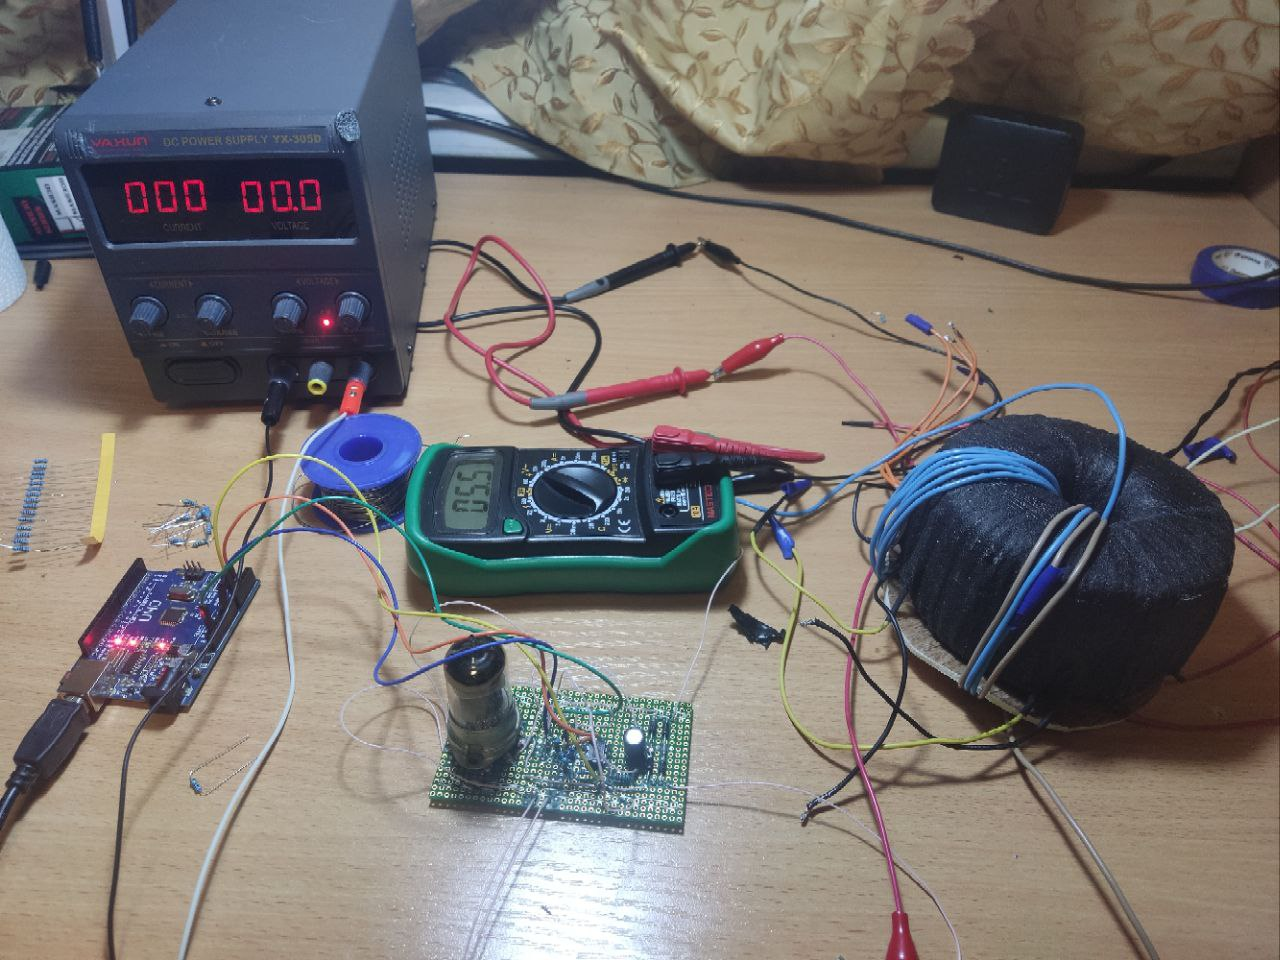
\includegraphics[scale=0.4]{photo.jpg}
    \caption{Экспериментальная установка}
    \label{fig:foto_ust}
\end{figure}


\newpage
\section{Ход работы}

Схема, представленная на рисунке рис.\ref{fig:scheme_ust}, используется для преобразования напряжения и тока между анодом и катодом в аналоговый сигнал, который подаётся на аналоговые порты Arduino UNO. В схеме используются резисторы и операционный усилитель для преобразования напряжения и тока в сигнал, допустимый для Arduino (входной сигнал - напряжение от 0 до 3.3 В с разрядностью 10 бит).\\

\underline{Измерение ВАХ между анодом и катодом триода при фиксированном напряжении накала:}

\begin{itemize}
    \item В сеть включается трансформатор с фиксированным напряжением, которое подается на схему к спирали накала, а также включается лабораторный блок питания, который питает лампу и Arduino UNO. В Arduino UNO предварительно загружен скрипт обработки сигнала с помощью Arduino IDE (скрипт  \ref{code_arduino}).
    \item Для чистоты эксперимента ожидается в среднем 5 мин. прогрев спирали накала (рис.\ref{fig:lamp}) для стабилизации ее температуры. В мониторе порта (Arduino IDE $\rightarrow$ Инструменты) выводятся значения напряжения и тока в реальном времени. В случае правильного подключения, при отсутствии напряжения на лабораторном блоке питания будет течь ток в лампе, что можно увидеть в потоке данных монитора порта (значения вида "0.0 0.10", слева напряжение, справа ток между анодом и катодом. Момент установления температуры будет, когда в потоке данных стабилизируется ток. Его значение в течении некоторого времени стремиться к определенному значению, которое соответствует конечной, установившейся температуре.
    \item После прогрева лампы производится очистка монитора порта, чтобы оставить только значения, снятые с момента установившегося тока между анодом и катодом. Далее, с помощью тонкой настройки напряжения на блоке питания(шаг 0.1 В) измеряется ВАХ на триоде. Каждое изменение напряжение должно быть зафиксировано в течении нескольких секунд для большего количества значений и как следствие получения средних значений(20-40 значений тока для каждого напряжения).
\end{itemize}

\underline{Снятие данных для множества напряжений накала:}

Для работы нужно получить для разных значений напряжения накала множество $\text{ВАХ}(U_{\text{накал}})$. На спираль подается напряжение от тороидального трансформатора преобразованное с 
помощью диодного моста и конденсатора. Путём добавления витков с помощью отдельного провода были получены напряжения от 3.3 В до 6 В с шагом 0.4 В на трансформаторе. 

Всего было проведено 28 измерений ВАХ для 7 опорных напряжений накала, на каждое напряжение был получен усредненный ВАХ 4 измерений(для минимизации погрешностей). Т.к. значения снимаются непрерывно во время эксперимента, то количество данных достигает >9000 точек для одного эксперимента. Поэтому итоговые ВАХи были обработаны в Python(код \ref{code_python}), усреднением каждой точки по значениям. Пример данных для ВАХ(4.3 В) представлен в таблице \ref{tab:data}.

Таким образом, были получено множество $\text{ВАХ}(U_{\text{накал}})$ для 7 напряжений накала.
 
\newpage
\section{Обработка результатов}

\par 
Теперь исследуем для каждого напряжения накаливания распределение электронов по скоростям. Для этого:

\begin{itemize}
    \item Построим c помощью программы обработки на Python (код программы \ref{code_python})
    построим график зависимости анодного тока от напряжения накала $\frac{dI}{dU}$  (рис. \ref{fig:graph_toka}).

    \begin{figure}[h!p]
    \centering
    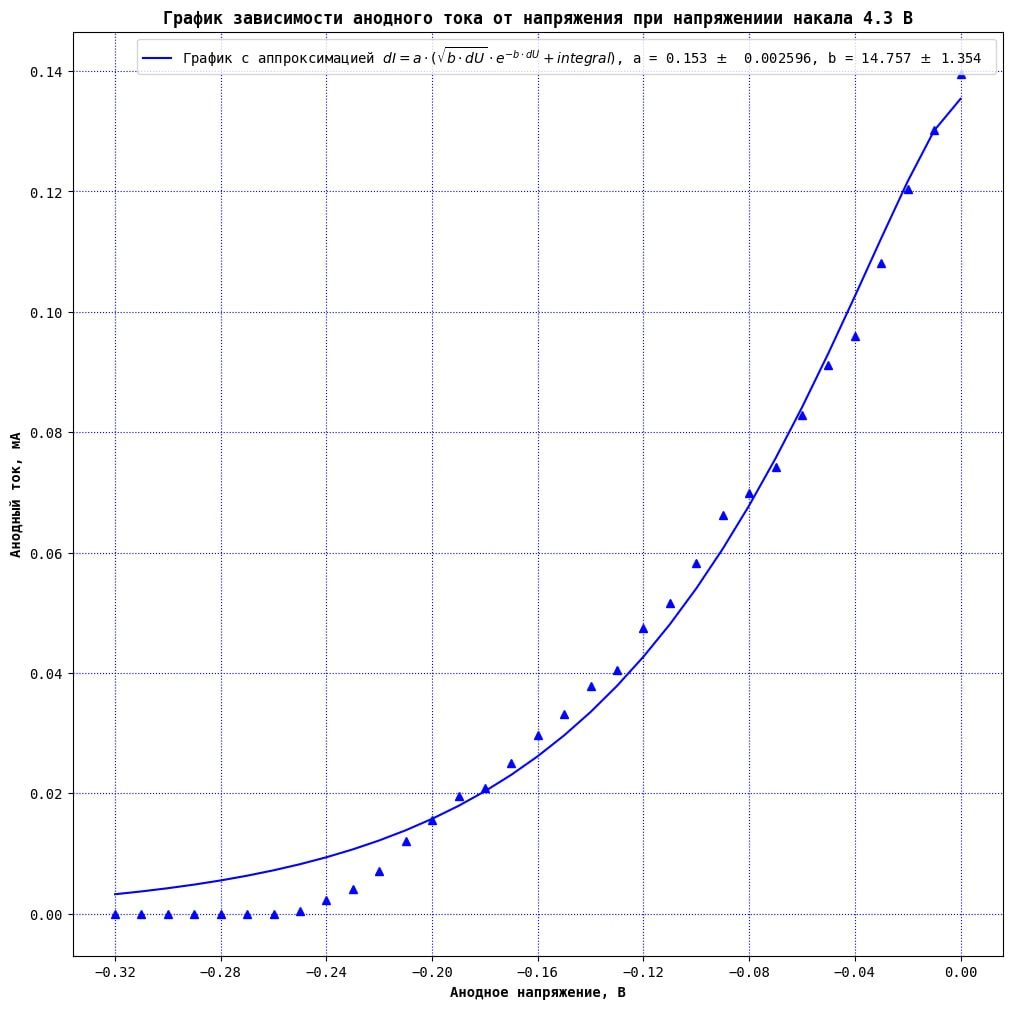
\includegraphics[scale=0.8]{ВАХ.jpg}
    \caption{График зависимости анодного тока от анодного напряжения}
    \label{fig:graph_toka}
    \end{figure}

    \newpage

    \item По предыдущему графику c помощью этой же программы (код программы \ref{code_python})
    построим график производной $\frac{dI}{dU}$ и аппроксимируем по формуле \ref{major_func} (рис. \ref{fig:graph_proizv}).
    \begin{figure}[h!p]
    \centering
    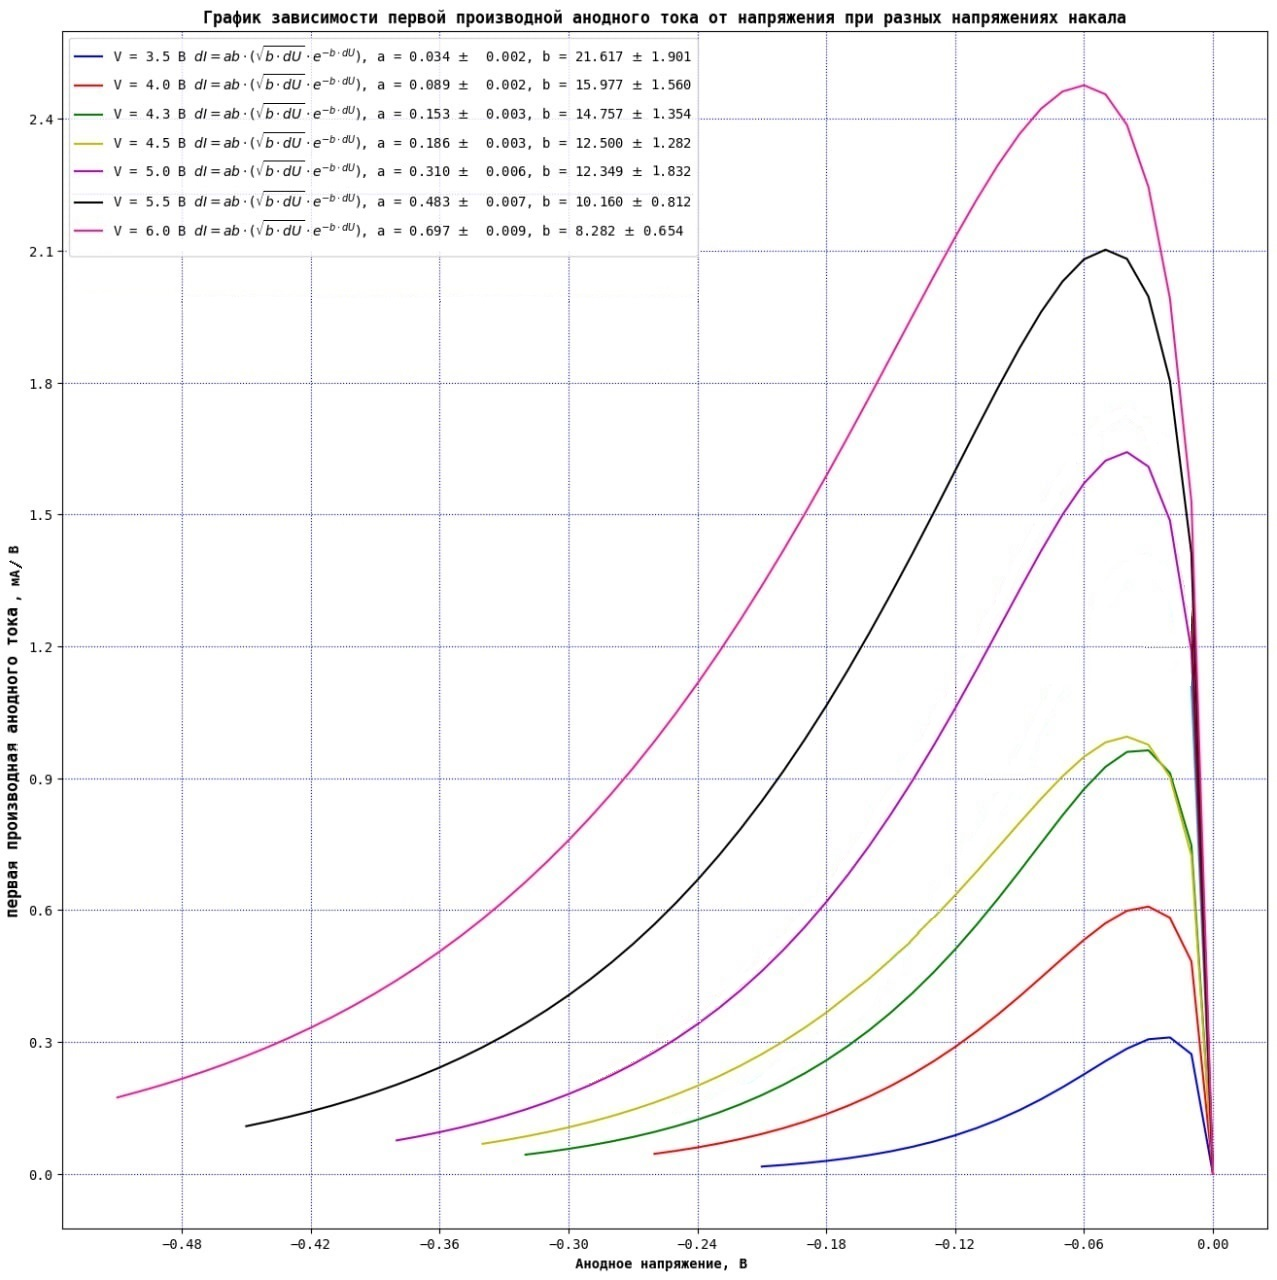
\includegraphics[scale=0.8]{dI_dU.jpg}
    \caption{График производной анодного тока от анодного напряжения}
    \label{fig:graph_proizv}
    \end{figure}

     Этот график является графиком плотности распределения термоэлектронов по энергиям с точностью до нормирующей константы.

     \newpage

    \item Построим в Desmos по вычисленным коэффициентам сам график плотности распределения, отнормировав его (рис.\ref{fig:graph_distr_dens}).


    \begin{figure}[h!p]
    \centering
    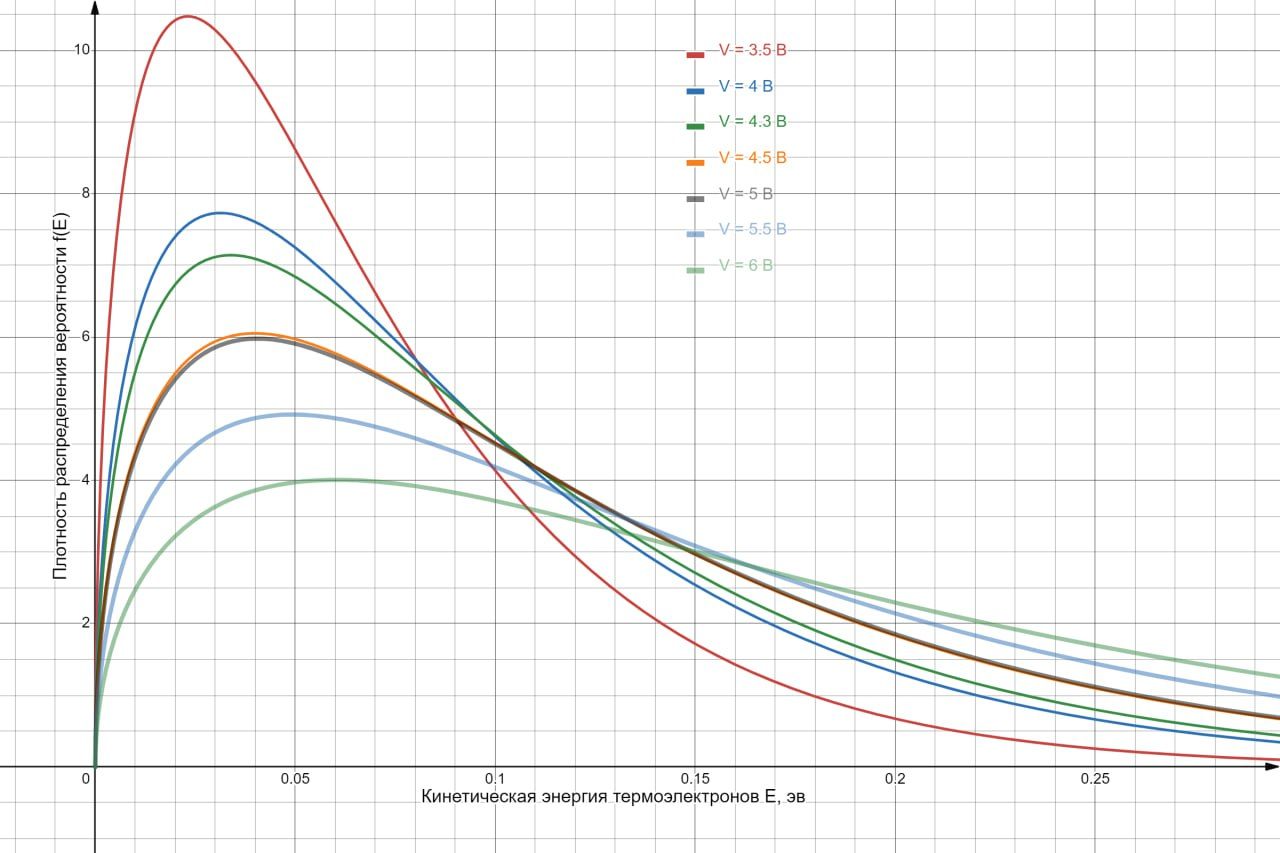
\includegraphics[scale=0.8]{distr_dens.jpg}
    \caption{График плотности распределения термоэлектронов по энергиям}
    \label{fig:graph_distr_dens}
    \end{figure}

    \newpage
    
    \item Зная плотность распределения по энергии $f(E)$, можно найти плотность
    распределения по модулю скорости $f_v(v)$, воспользовавшись соотношениями:
    
    \begin{equation}
        f(E)dE = f_v(v)dv, Е = mv^2/2, dE = mvdv,
    \end{equation}

    Тогда
    \begin{equation}
        f_v(v) = f(E) \cdot dE/dv = f(E) \cdot mv = f(E) \cdot \sqrt{2mE}
    \end{equation}

    Построим в Desmos график плотности распределения электронов по скоростям для разных напряжений (рис. \ref{fig:veloc_distr}).

    \begin{figure}[h!p]
    \centering
    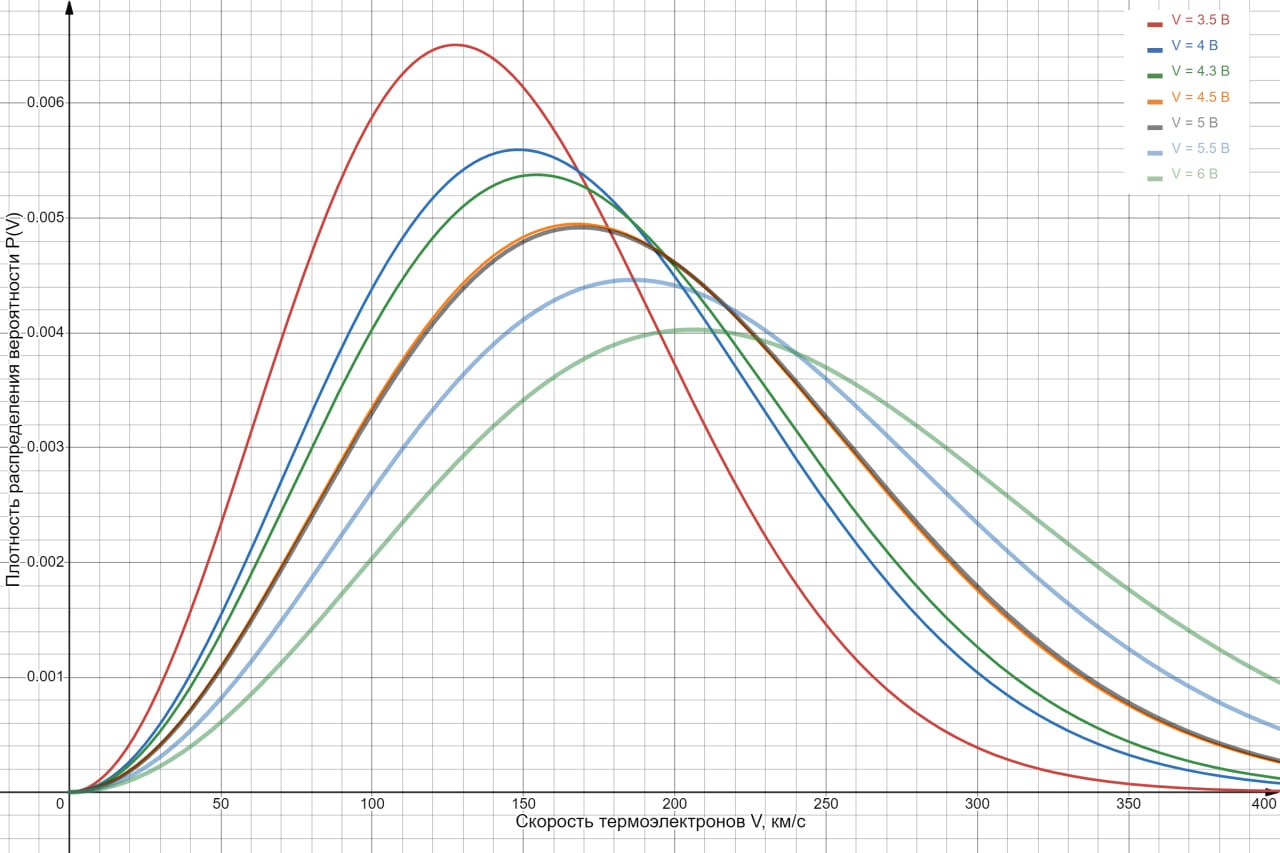
\includegraphics[scale=0.8]{veloc_distr.jpg}
    \caption{График плотности распределения термоэлектронов по скоростям}
    \label{fig:veloc_distr}
    \end{figure}

    \newpage

    \item Взяв производную от плотности распределения скорости по скорости и приравняв к нулю:
    
    \begin{equation}
        \frac{a b \sqrt{b x} \left(- b x + 1\right) e^{- b x}}{\sqrt{x}} = 0
    \end{equation}
    
    Найдём экстремум плотности распределения по скоростям - это и будет наша наивероятнейшая скорость, по этим скоростям вычислим температуры электронов.
    \par
    Данные представлены в таблице:

\begin{table}[!ht]
\centering
\begin{tabular}{|c|c|c|c|c|}
\hline
Напряжение $U$, В & Скорость $v$, м/с & \begin{tabular}[c]{@{}c@{}}Погрешность \\ скорости $dv$, м/с\end{tabular} & Температура $T$, $K$ & \begin{tabular}[c]{@{}c@{}}Погрешность \\ температуры $dT$, $K$\end{tabular} \\ \hline
3,5             & 128             & 11                                                                       & 536              & 47                                                                       \\ \hline
4,0               & 148             & 14                                                                       & 726              & 71                                                                       \\ \hline
4,3             & 154             & 14                                                                       & 786              & 72                                                                       \\ \hline
4,5             & 168             & 17                                                                       & 928              & 95                                                                       \\ \hline
5,0               & 169             & 25                                                                       & 939              & 139                                                                      \\ \hline
5,5             & 186             & 15                                                                       & 1141             & 91                                                                      \\ \hline
6,0               & 206             & 16                                                                       & 1400             & 111                                                                      \\ \hline
\end{tabular}
\caption{Скорости и температуры электронов для различных напряжений}
\label{tab:result}
\end{table}

    По этим данным построим в SciDavis график зависимости температуры от напряжения (рис.\ref{fig:result}).
    
    \begin{figure}[h!p]
    \centering
    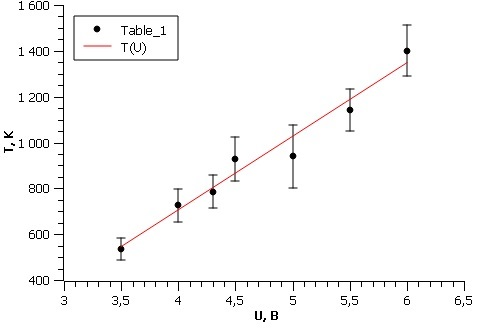
\includegraphics[scale=1.2]{result.jpg}
    \caption{График зависимости температуры термоэлектронов от напряжения}
    \label{fig:result}
    \end{figure}

    Эта зависимость должна быть линейной, так как, если принять, что темлообмен между нитью накаливания и окружающей средой (вакуум) происходит только засчёт термоэлектронов (пренебрегая рассеиванием тепла из-за излучения), то :

    \begin{equation}
        \frac{U^2}{R} \sim \varkappa \cdot T \sim T^2 \rightarrow T \sim U,
    \end{equation}
    считая, что коэффициент теплопроводности $\varkappa = \alpha \cdot T$ и постоянным сопротивление(в прогревшемся состоянии). 

\end{itemize}

\newpage
\section{Выводы}

Экспериментальным путём были получены плотности распределения термоэлектронов по скоростям. Они подтверждают наше предположения о максвелловском распределении электронов, вылетающих из нити накала. 
Подобно тому как обычный газ представляет собой совокупность большого количества  свободных молекул, электронный газ создаётся ансамблем электронов в некотором объёме.

\par 
Многие характеристики молекулярного газа, такие как плотность распределения частиц по энергии, вводятся и применительно к электронному газу, хотя выражения для них отличаются от случая обычных газов.

\par 
По данным распределениям были получены температуры движения термоэлектронов, находящиеся в диапазоне: 500 - 1400 К для различных напряжений. 
\par
На точность температуры повлияли в основном два фактора: наличие элетронного облака в триоде и контактной разности потенциалов в системе катод-анод.


\newpage
\section{Приложения}

\subsection{Таблицы}

\begin{table}[!ht]
\centering
\caption{Данные усредненной ВАХ для 4.3 В}
\begin{tabular}{|c|c|}
\hline
Напряжение, В & Ток, мА \\ \hline
0.25          & 0.000   \\ \hline
0.24          & 0.002   \\ \hline
0.23          & 0.004   \\ \hline
0.22          & 0.007   \\ \hline
0.21          & 0.012   \\ \hline
0.20          & 0.016   \\ \hline
0.19          & 0.020   \\ \hline
0.18          & 0.021   \\ \hline
0.17          & 0.025   \\ \hline
0.16          & 0.030   \\ \hline
0.15          & 0.033   \\ \hline
0.14          & 0.037   \\ \hline
0.13          & 0.040   \\ \hline
0.12          & 0.047   \\ \hline
0.11          & 0.052   \\ \hline
0.10          & 0.058   \\ \hline
0.09          & 0.066   \\ \hline
0.08          & 0.070   \\ \hline
0.07          & 0.074   \\ \hline
0.06          & 0.083   \\ \hline
0.05          & 0.091   \\ \hline
0.04          & 0.096   \\ \hline
0.03          & 0.108   \\ \hline
0.02          & 0.120   \\ \hline
0.01          & 0.130   \\ \hline
\end{tabular}
\label{tab:data}
\end{table}


\newpage
\subsection{Фотографии и графики}

\begin{figure}[h!p]
    \centering
    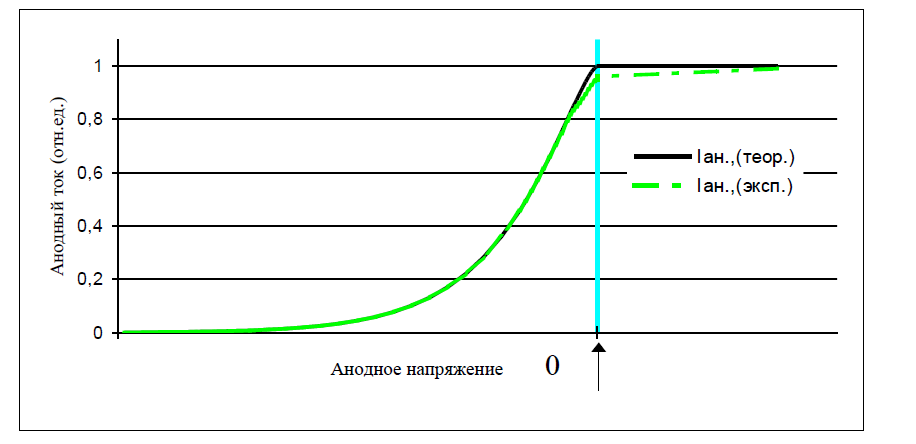
\includegraphics[scale=0.8]{image1.png}
    \caption{Зависимость анодного тока диода от напряжения между анодом и катодом в вакуумном диоде (теория и
эксперимент).}
    \label{fig:zavis_toka}
\end{figure}

\begin{figure}[h!p]
    \centering
  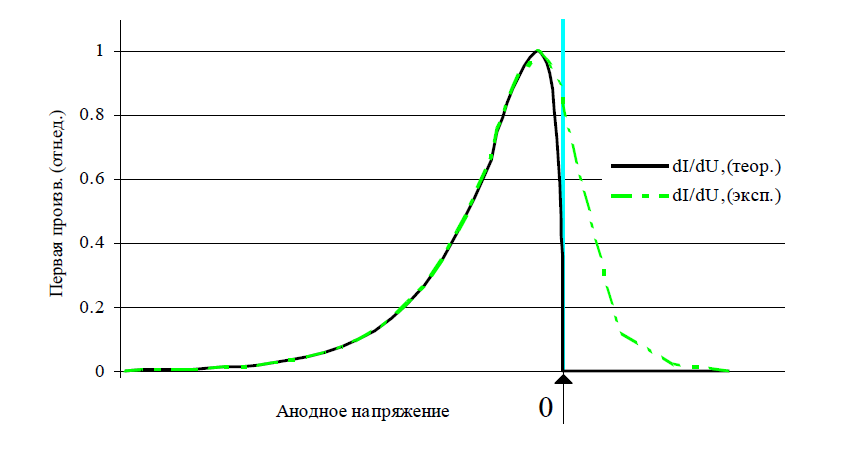
\includegraphics[scale=0.9]{image2.png}
   \caption{Зависимость первой производной анодного тока по анодному напряжению dIан/dUан от
напряжения между анодом и катодом в вакуумном диоде (теория и эксперимент).}
    \label{fig:zavis_proizv}
\end{figure}

\begin{figure}[h!p]
    \centering
    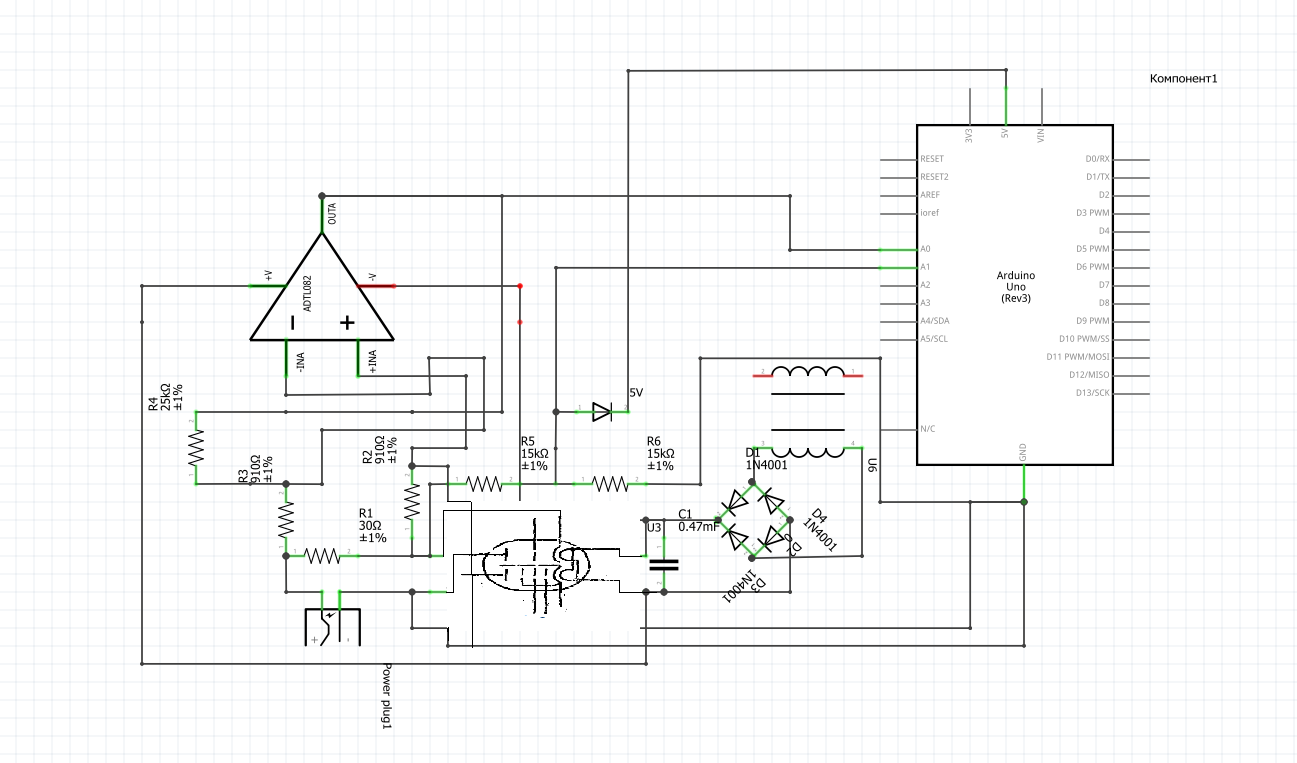
\includegraphics[scale=0.7]{схема.png}
    \caption{Схема установки}
    \label{fig:scheme_ust}
\end{figure}

\begin{figure}[h!p]
    \centering
    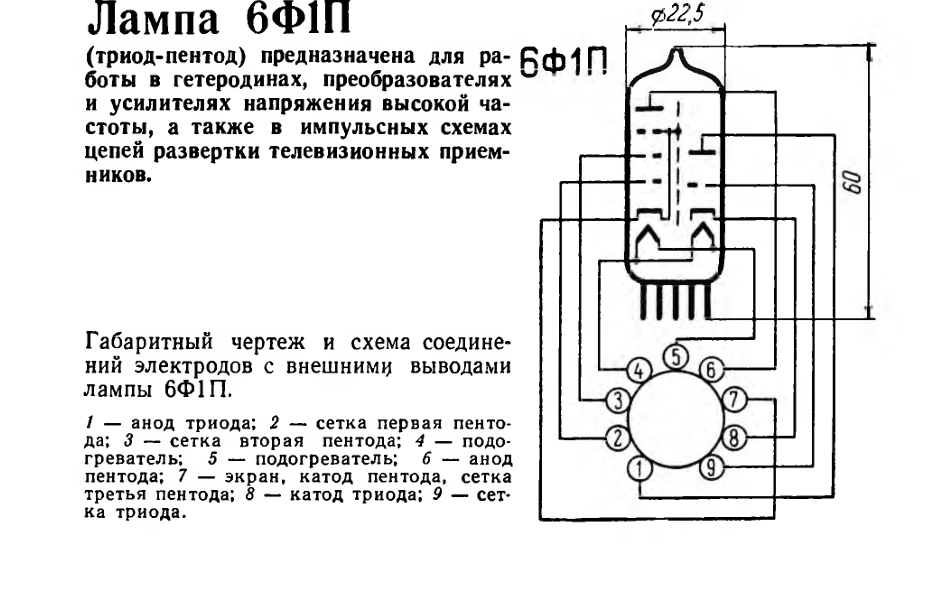
\includegraphics[scale=0.55]{image.png}
    \caption{Распиновка лампы 6Ф1П}
    \label{fig:ref_6f1p}
\end{figure}

\begin{figure}[h!p]
    \centering
    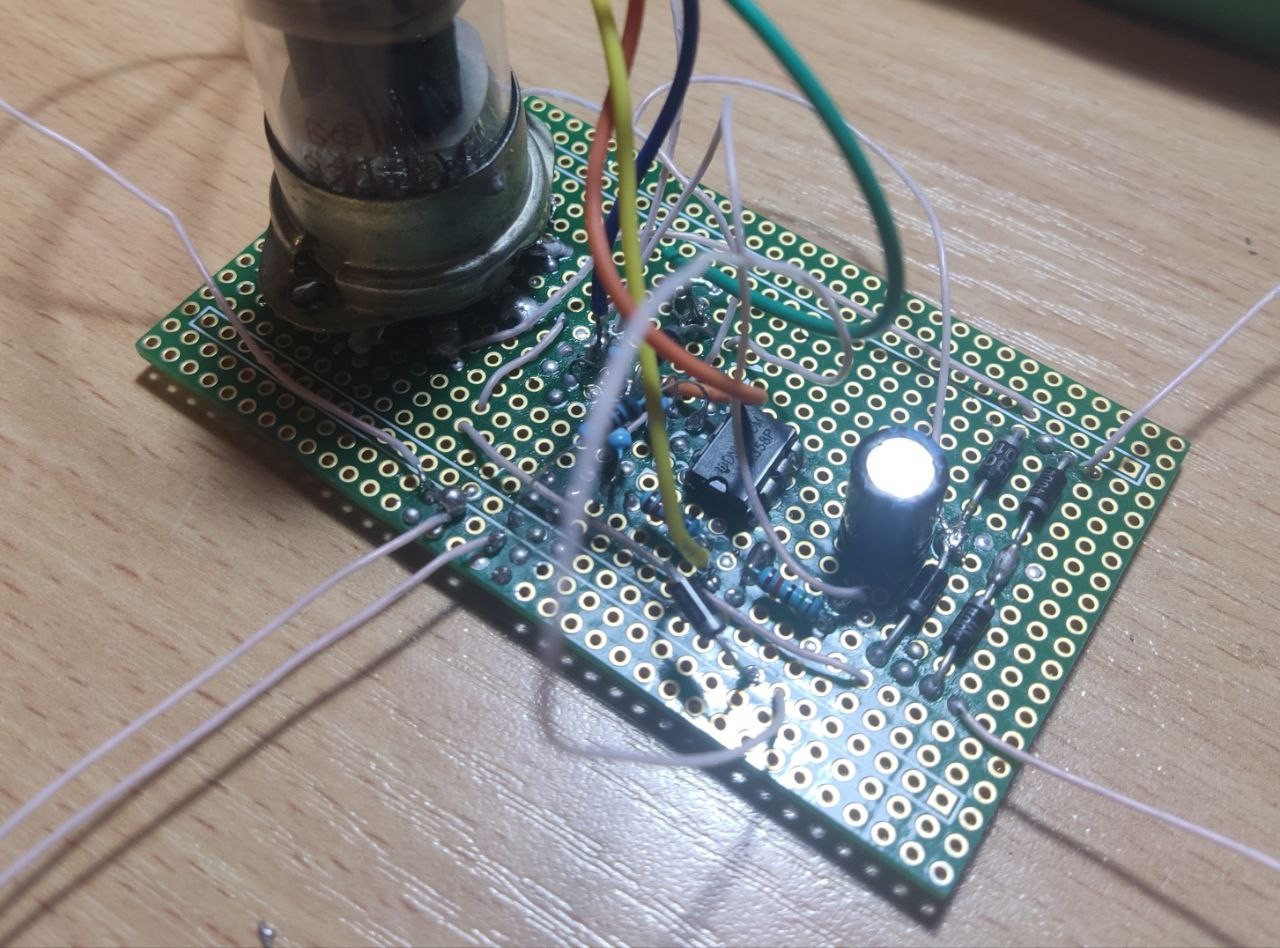
\includegraphics[scale=0.35]{photo2.jpg}
    \caption{Плата}
    \label{fig:plata}
\end{figure}

\begin{figure}[h!p]
    \centering
    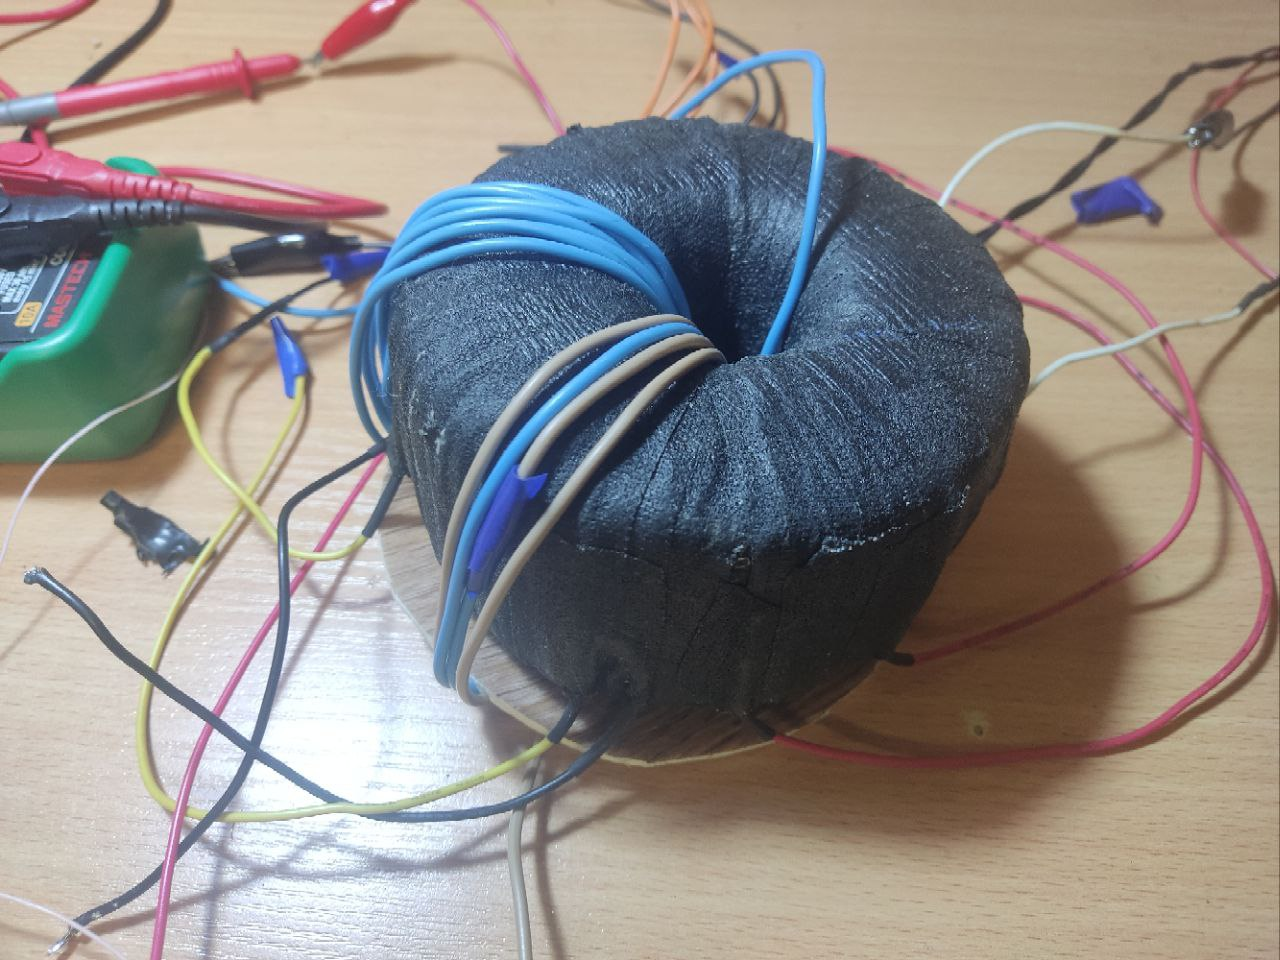
\includegraphics[scale=0.35]{photo3.jpg}
    \caption{Тороидальный трансформатор}
    \label{fig:transformator}
\end{figure}

\begin{figure}[h!p]
    \centering
    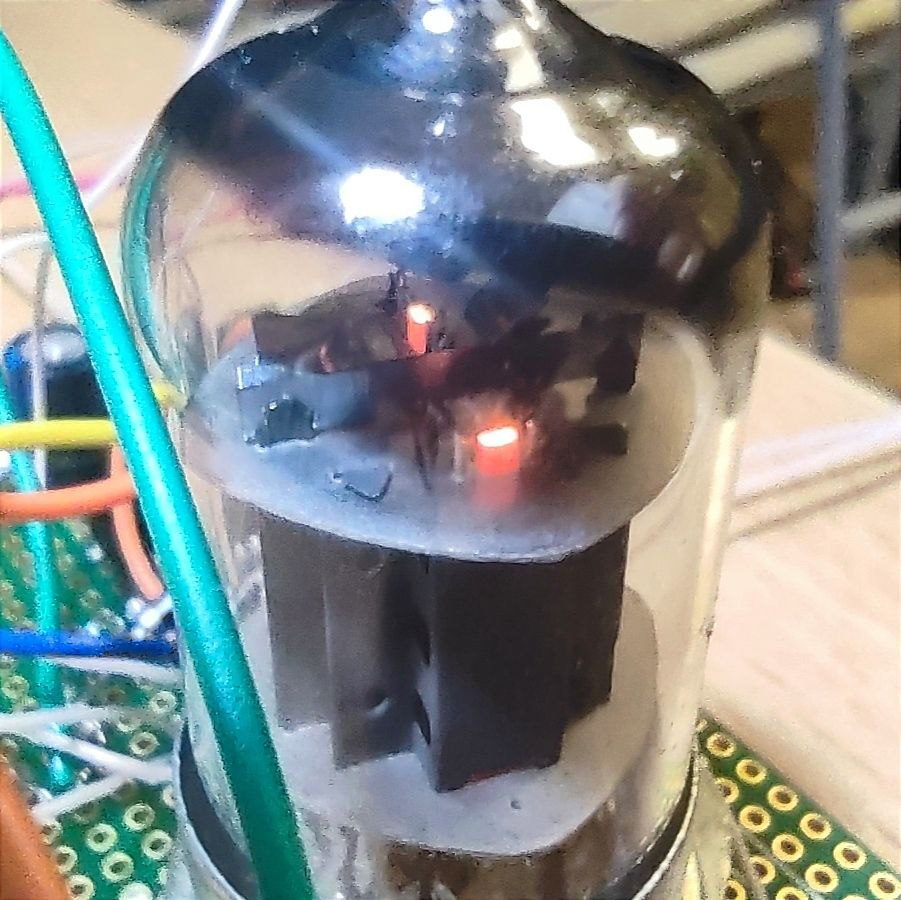
\includegraphics[scale=0.4]{photo1.jpg}
    \caption{Спираль накаливания}
    \label{fig:lamp}
\end{figure}

\newpage
\subsection{Исходный код}

\vspace{15pt}

\subsubsection{Код для обработки данных с Arduino} \label{code_arduino}

\begin{lstlisting}

#define voltageAC_pin A0
#define voltageShunt_pin A1
#define Shunt 30.0f

float voltageAC    = 0;
float voltageShunt = 0;

void setup() {
  Serial.begin(9600);
  pinMode(voltageAC_pin, INPUT);
  pinMode(voltageShunt_pin, INPUT);
}

float getCurrent() {
  return analogRead(voltageShunt_pin) / 1024.0f * 5.0f * 1000.0f / (150000.0f + 910.0f) * 910.0f / Shunt;
}

float getVoltage() {
  return analogRead(voltageAC_pin) / 1024.0f * 5.0f * 2.0f;
}

bool voltage[1024] = {0};

void loop() {
  int value = analogRead(voltageAC_pin);
  if(voltage[value] < 2) {
      voltage[value] =  voltage[value] + 1;
      Serial.print(getVoltage());
      Serial.print("; ");
      Serial.println(getCurrent());
  }
}

\end{lstlisting}

\newpage
\subsubsection{Код для построения графика с помощью Matplotlib} \label{code_python}

\begin{lstlisting} 

import matplotlib.pyplot as plt                         #include libs  <DONT CHANGE>
import matplotlib.ticker as ticker
from scipy.optimize import curve_fit
from IPython.display import display, Math, Latex
import numpy as np
import math as mth
import scipy.special

import warnings
warnings.filterwarnings("ignore")

plt.rcParams["font.family"] = "monospace"

def mapping(x, a, b):                #Function of approximating give to curve_fit <TO CHANGE!!!>
    new_arr = []
    for x_i in x:
        new_arr.append(a*(mth.sqrt(abs(x_i)*abs(b))*mth.exp(-abs(x_i)*abs(b)) + mth.sqrt(mth.pi) * scipy.special.erfc(mth.sqrt(abs(x_i)*abs(b))) / 2))
    return new_arr

def mapping_1(x, a, b):                #Function of approximating give to curve_fit <TO CHANGE!!!>
    new_arr = []
    for x_i in x:
        new_arr.append(a*b*(mth.sqrt(abs(x_i)*abs(b))*mth.exp(-abs(x_i)*abs(b))))
    return new_arr

save_pic = "./graphic.png"

#==================================================================================================
_, ax = plt.subplots(figsize=(12, 12))
ax.xaxis.set_major_locator(ticker.MaxNLocator(10))
ax.xaxis.set_minor_locator(ticker.MaxNLocator(10))
ax.yaxis.set_major_locator(ticker.MaxNLocator(10))
ax.yaxis.set_minor_locator(ticker.MaxNLocator(10))

ax.set_xlabel("Napryazhenie", fontweight="bold")
ax.set_ylabel("Tok", fontweight="bold")
ax.set_title("Graphic", fontweight="bold")

plt.grid(color="blue", visible=True, which='major',axis='both',alpha=1, linestyle = ":")
plt.grid(color="blue", visible=True, which='minor',axis='both',alpha=1, linestyle = ":")
#==================================================================================================
dy_dx = []
#processing data

x = []
y = []
file = open('data3.3v.txt', 'r')                 #open file with data
while (line := file.readline()):              # every line have x, y, y1 ...
  s = line.split('; ')
  if (len(s) != 0):
    x.append(float(s[0].replace(',','.'))*(-1)) #collect in x[] y1[] y2[] with change "," -> "." (if excel)
    y.append(float(s[1].replace(',','.')))

for i in range(1, len(x)):
  for j in range(len(x) - i):
    if (x[j] > x[j+1]):
      x[j], x[j+1] = x[j+1], x[j]
      y[j], y[j+1] = y[j+1], y[j]


print(x)

z = []
cool_x = []
cool_y = []

for i in range(1, len(x)):
  if (x[i-1] == x[i]):
    z.append(y[i - 1])
    continue
  if (len(z) > 0):
    z.append(y[i - 1])
    cool_x.append(x[i-1])
    cool_y.append(sum(z) / len(z))
    z = []
    continue
  cool_x.append(x[i - 1])
  cool_y.append(y[i - 1])

if (len(z) > 0):
  z.append(y[len(x) - 1])
  cool_x.append(x[len(x)-1])
  cool_y.append(sum(z) / len(z))
  z = []
else:
  cool_x.append(x[len(x) - 1])
  cool_y.append(y[len(x) - 1])

xData = np.array(cool_x, dtype=float)
yData = np.array(cool_y, dtype=float)

dy_dxData = np.array(dy_dx, dtype=float)

init_param = np.array([1.0, 1.0])

covs   = []
coeffs = []
coeffs, covs = curve_fit(mapping, cool_x, cool_y, init_param) #give func and our measurements
print(coeffs)
print(covs)
deviation = np.sqrt(np.diag(covs))

yFitData = mapping(cool_x, *coeffs)  #it returns array of aproximating coeffs <CHANGE DEPEND OF FUNC>

plt.plot(cool_x, cool_y, 'b^') #approximating praphic
plt.plot(cool_x, yFitData, color = 'b', label = f"Graphic") #approximating praphic

# yFitData = mapping_1(xData, *coeffs)

x = []
y = []


#=======================================================================================
for i in range(len(cool_x)-1):
  if ((cool_x[i+1]-cool_x[i]) != 0):
    dy_dx.append(float(cool_y[i+1]-cool_y[i])/float(cool_x[i+1]-cool_x[i]))

file2 = open('cool.txt', 'w')                 #open file with data
for i in range(len(cool_x)-1):
  file2.write(str(cool_x[i]) + '\t' + str(cool_y[i]) + '\n')

#plt.plot(cool_x, dy_dx, 'm*', label='')
#========================================================================================

plt.legend()
plt.show()
plt.savefig(save_pic)
file2.close()
file.close()

\end{lstlisting}


\newpage
\section{Список литературы}
\begin{itemize}
    \item Сивухин Д. В. Общий курс физики. Т. II. Термодинамика и молекулярная физика - М.: Физматлит, 2021.
    \item Овчинкин В.А. Лекции по термодинамике и молекулярной физике. - М.: Физматкнига, 2023.
\end{itemize}


%foto
%\begin{figure}[!p]
%    \centering
%    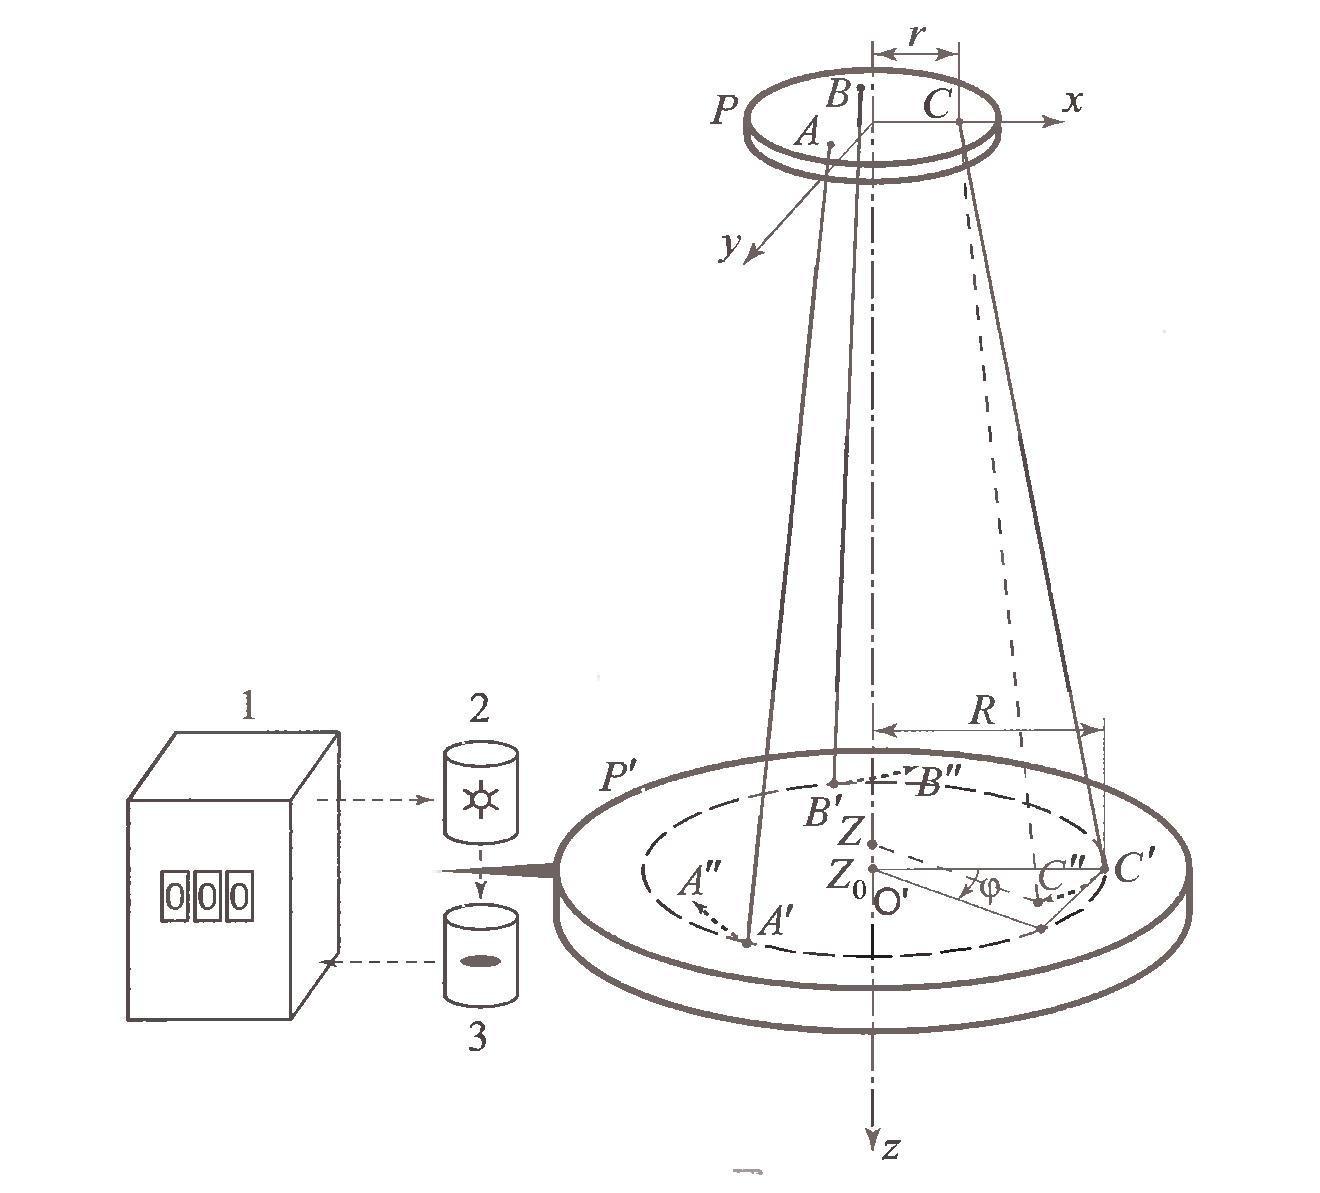
\includegraphics[scale=0.15]{foto.jpg}
%    \caption{ПНазвание}
%    \label{fig:ref_to_this_foto}
%\end{figure}

%table
%\begin{table}[!ht]
%    \centering
%    \begin{tabular}{}
%    ...
%    \end{tabular}
%    \caption{Название}
%    \label{fig:table_to_this_foto}
%\end{table}